\chapter{Evaluation}
\label{chap:eval}

% Our sampling data for testing our application were especially highly textured images of sculptures.
Highly textured surfaces are especially suitable for detecting SIFT and SURF features since they typically provide a large number of visually distinct ``blobs'' in their photo. 
For this reason, we chose two such objects for our testing datasets. 
The two pairs of photos are shown in Figure \ref{fig:input_samples}. 
The photos were taken by the Sony ST27i device.

\begin{figure}[H]
\centering

\begin{subfigure}[b]{0.45\textwidth}
\centering
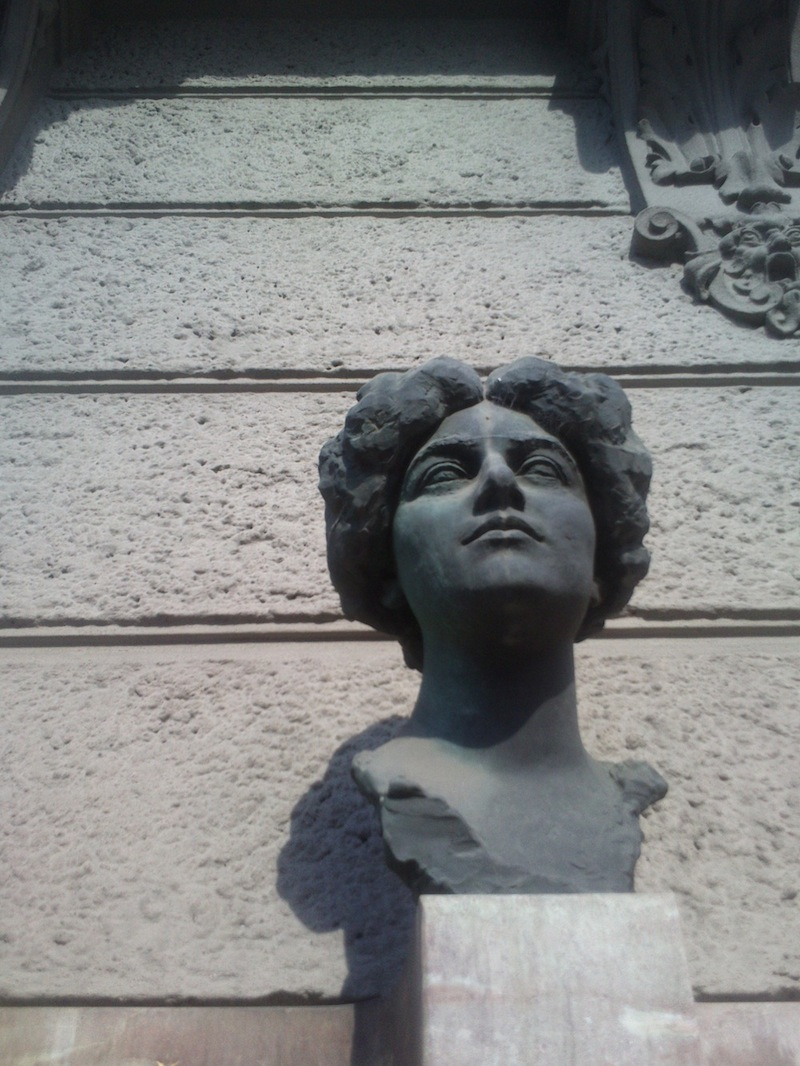
\includegraphics[width=6.0cm]{img/ema_a.png}
\caption{The left image of a bust of Ema Destinová.} \label{0}
\end{subfigure}
\begin{subfigure}[b]{0.45\textwidth}
\centering
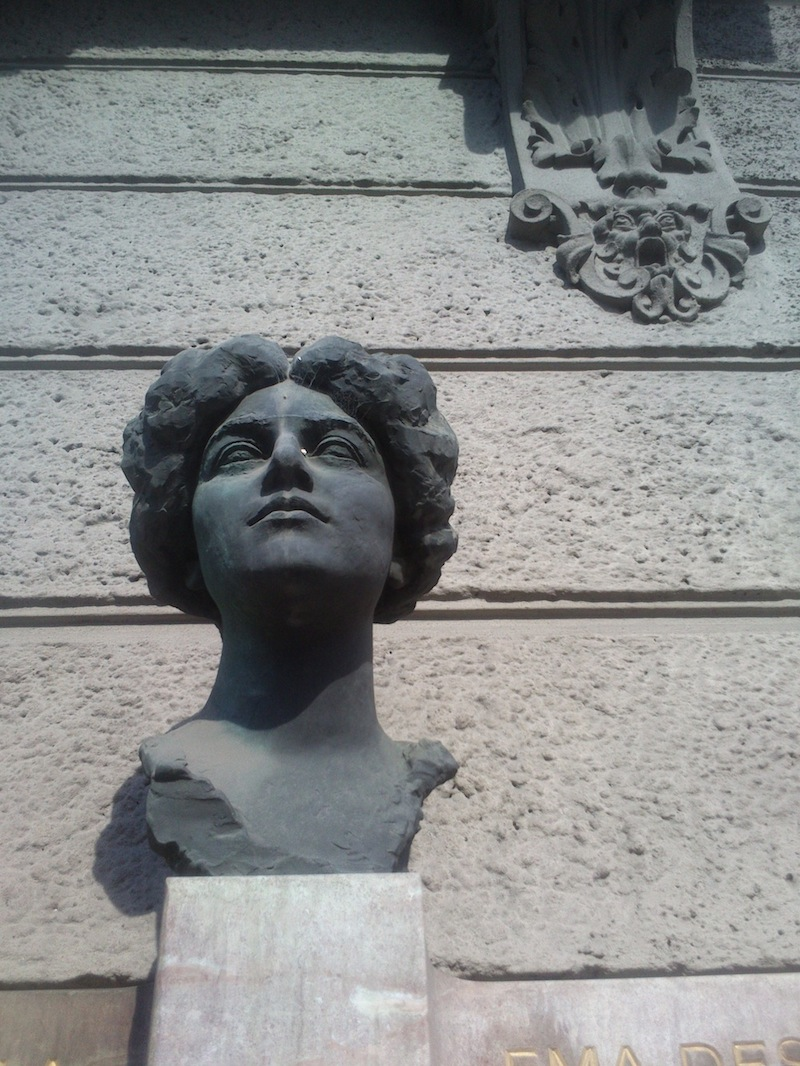
\includegraphics[width=6.0cm]{img/ema_b.png}
\caption{The right image of a bust of Ema Destinová.} \label{2}
\end{subfigure}
\begin{subfigure}[b]{0.45\textwidth}
\centering
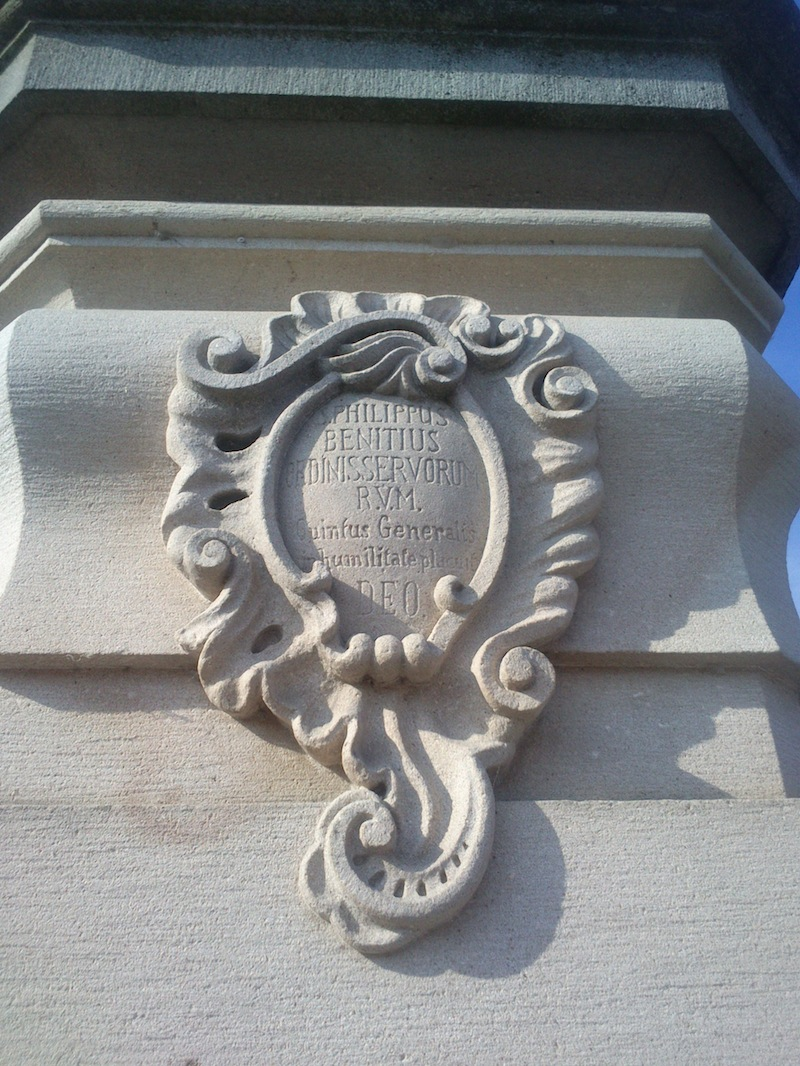
\includegraphics[width=6.0cm]{img/memorial_a.png}
\caption{The left image of a memorial.} \label{3}
\end{subfigure}
\begin{subfigure}[b]{0.45\textwidth}
\centering
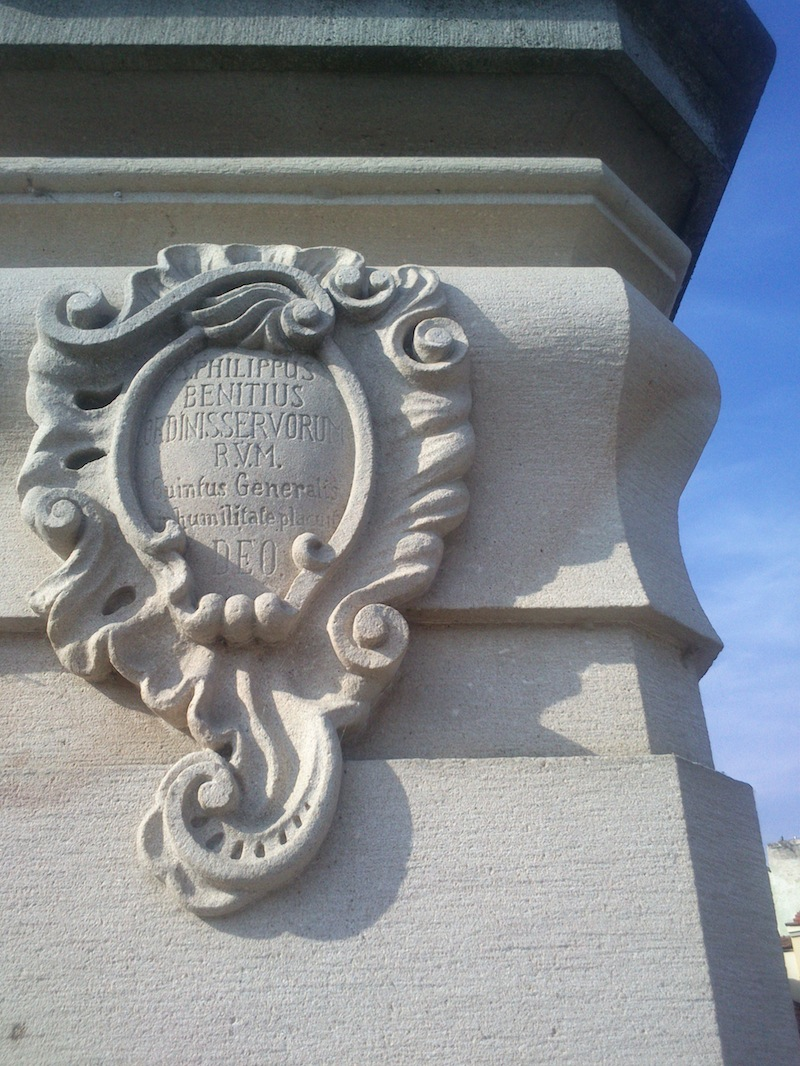
\includegraphics[width=6.0cm]{img/memorial_b.png}
\caption{The right image of a memorial.} \label{4}
\end{subfigure}

\caption[]{Testing datasets.} 
\label{fig:input_samples}
\end{figure}

\section{Results}

For the testing input shown in Figure \ref{fig:input_samples}, the results seem satisfying. 
The SURF detector detects a sufficient number of features and after filtering there remain enough good matches to get the information about the depth of some parts of the input images, see to Figure \ref{fig:matching}.

\begin{figure}[H]
\centerline{
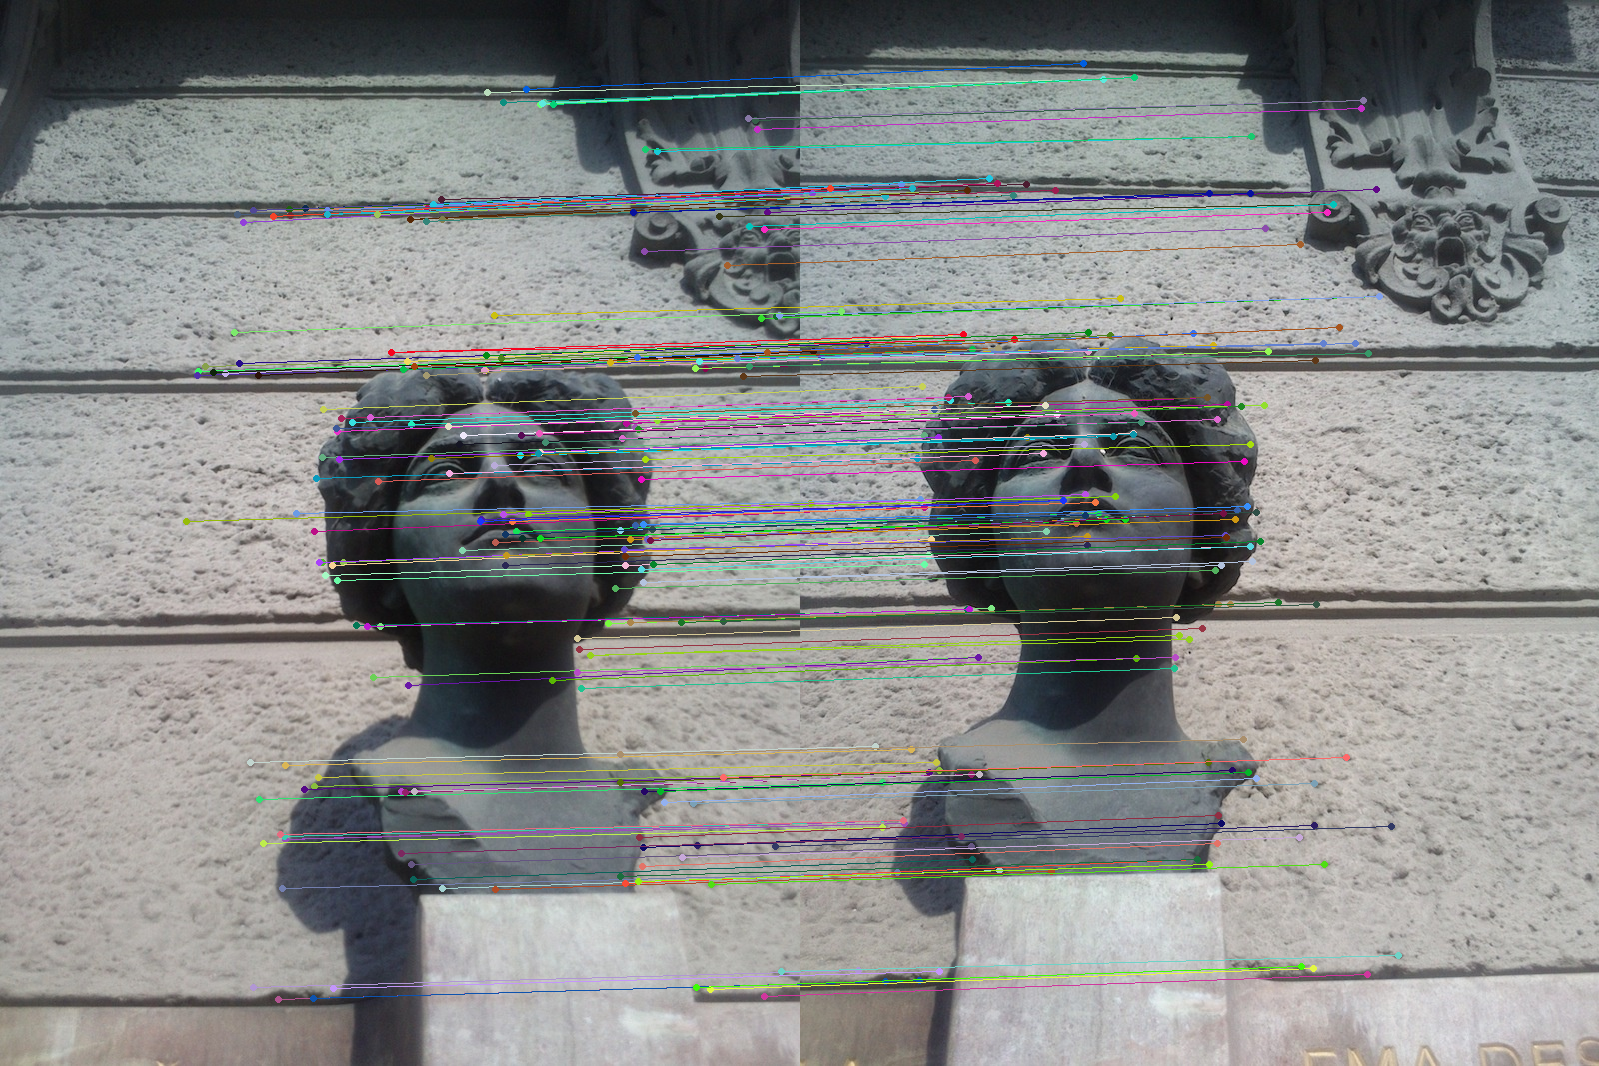
\includegraphics[width=14.0cm]{img/ema_matching.png}}
\centerline{
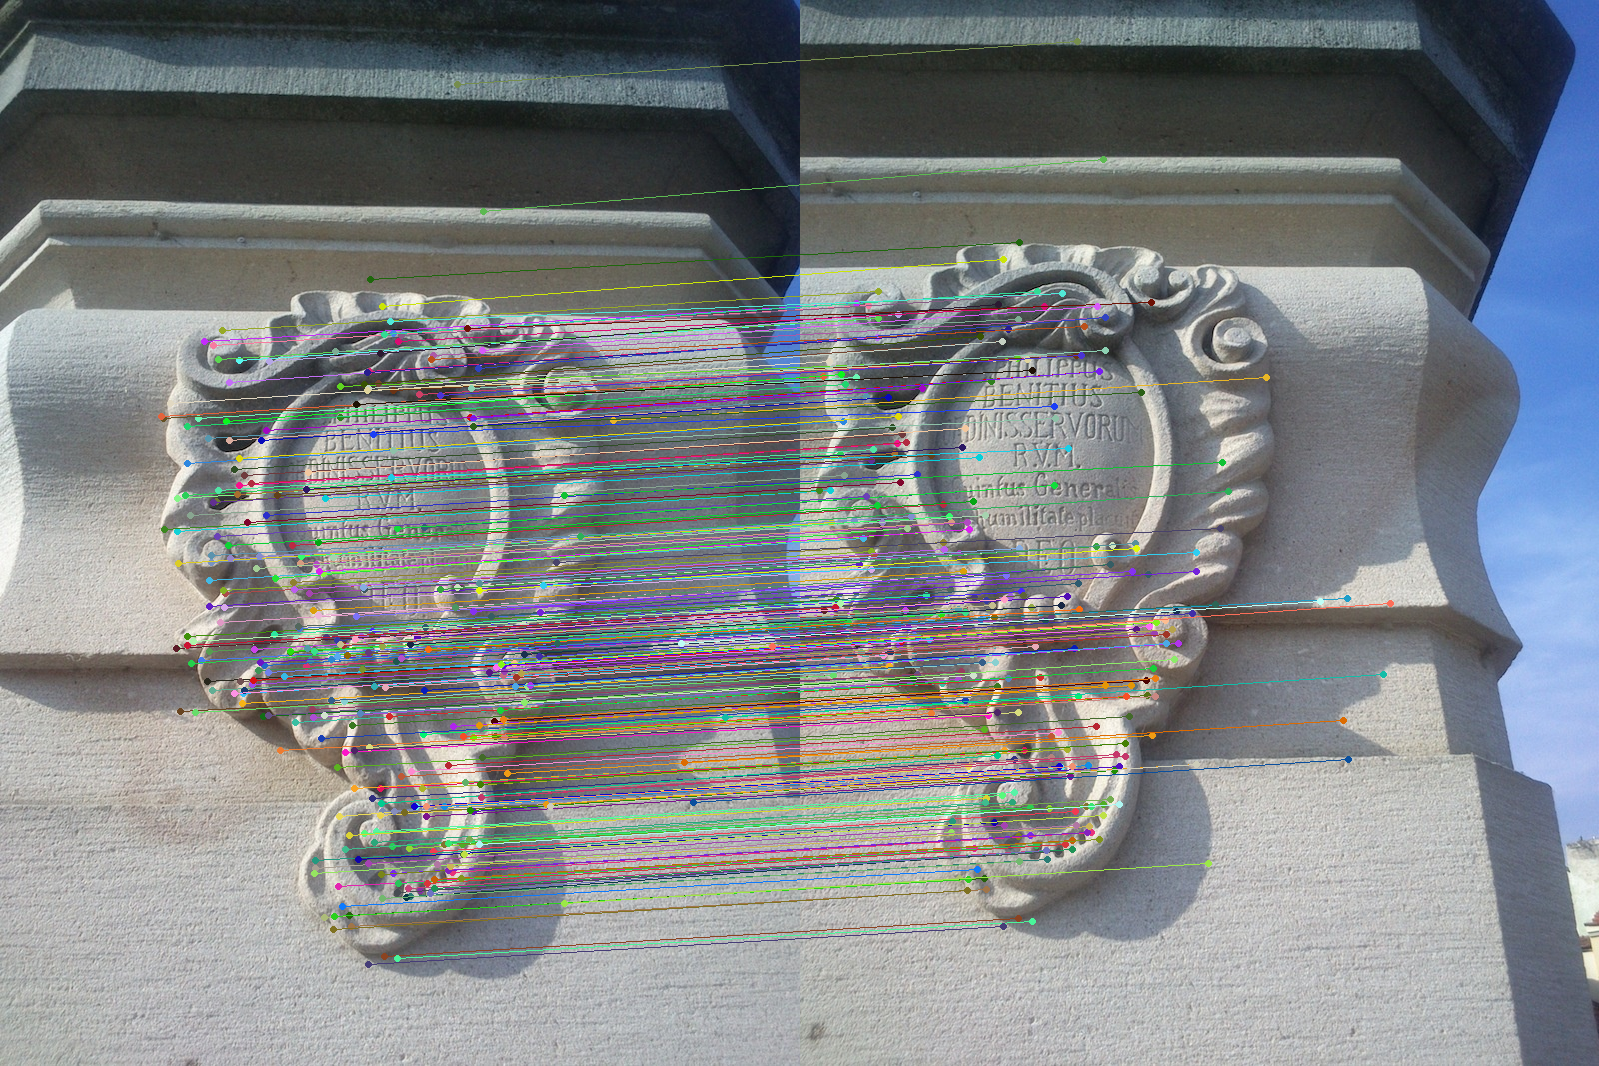
\includegraphics[width=14.0cm]{img/memorial_matching.png}}
\caption{The results of SURF matching -- corresponding points are connected using line segments.}
\label{fig:matching}
\end{figure}

For the pair of images of the bust of Ema Destinová, we get a 3D model of the textured parts of the head and a part of the wall in the background.
The second pair gives us a result in the form of an inclined plane in the angle of the memorial in the picture.
These results are compatible with the actual appearance of the scenes.

\begin{figure}[H]
\centerline{
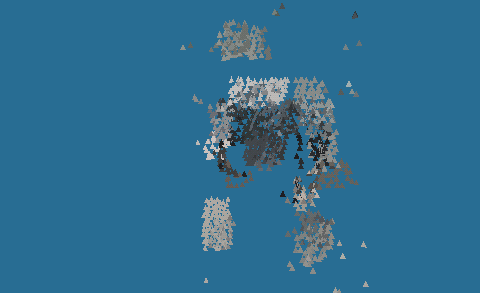
\includegraphics[width=6.5cm]{img/ema_3Dresult.png}
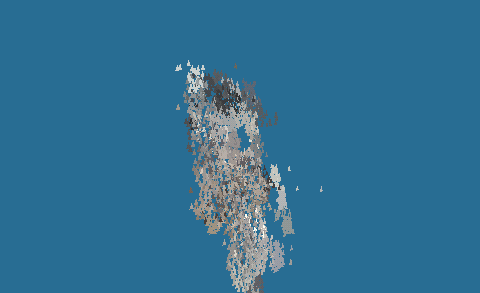
\includegraphics[width=6.5cm]{img/memorial_3Dresult.png}}
\caption{The output as a 3D model. The model of Ema Destinová's sculpture (left) and of a memorial (right).}
\label{fig:outupt_samples}
\end{figure}

On the other hand for images with noise or images without textures, the matching typically results in a series of mismatches so the 3D model does not correspond with the reality.
An example of such input is shown in Figure \ref{fig:bad_example}.

\begin{figure}[h]
\centering

\begin{subfigure}[b]{0.45\textwidth}
\centering
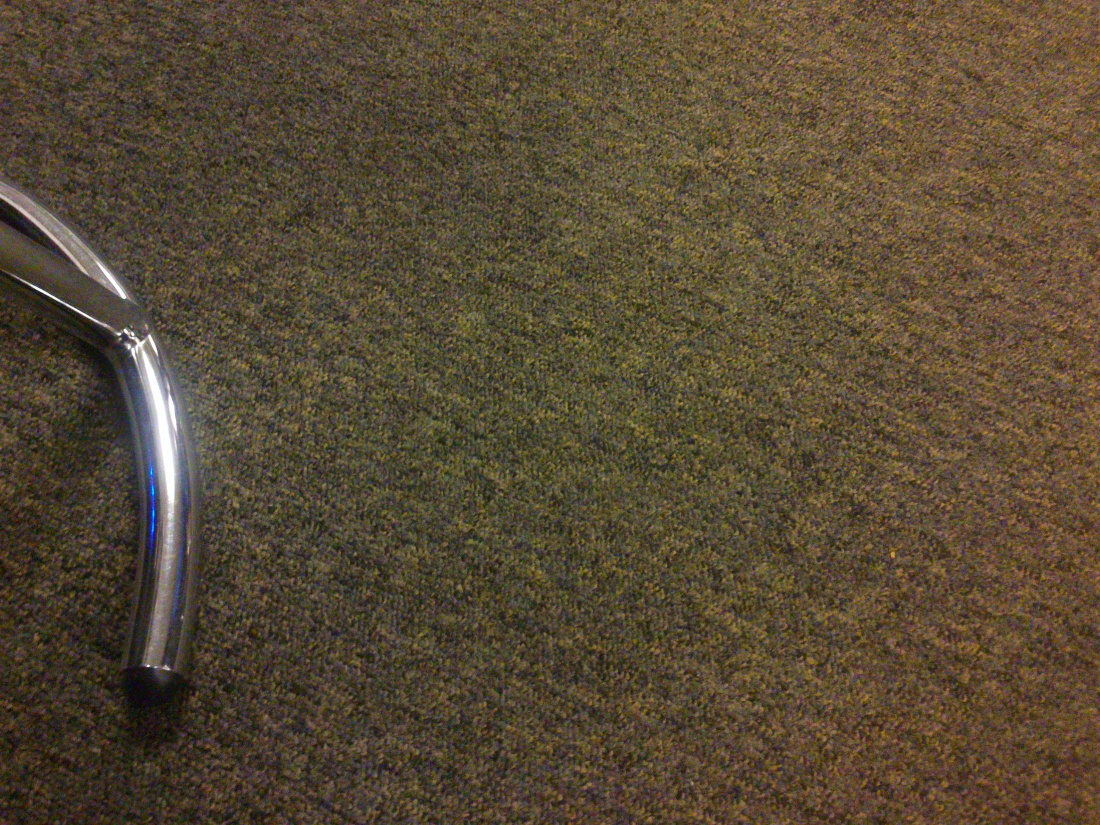
\includegraphics[width=4.5cm]{img/bad_input1.png}
\caption{The left image of the input image.} \label{x0}
\end{subfigure}
\begin{subfigure}[b]{0.45\textwidth}
\centering
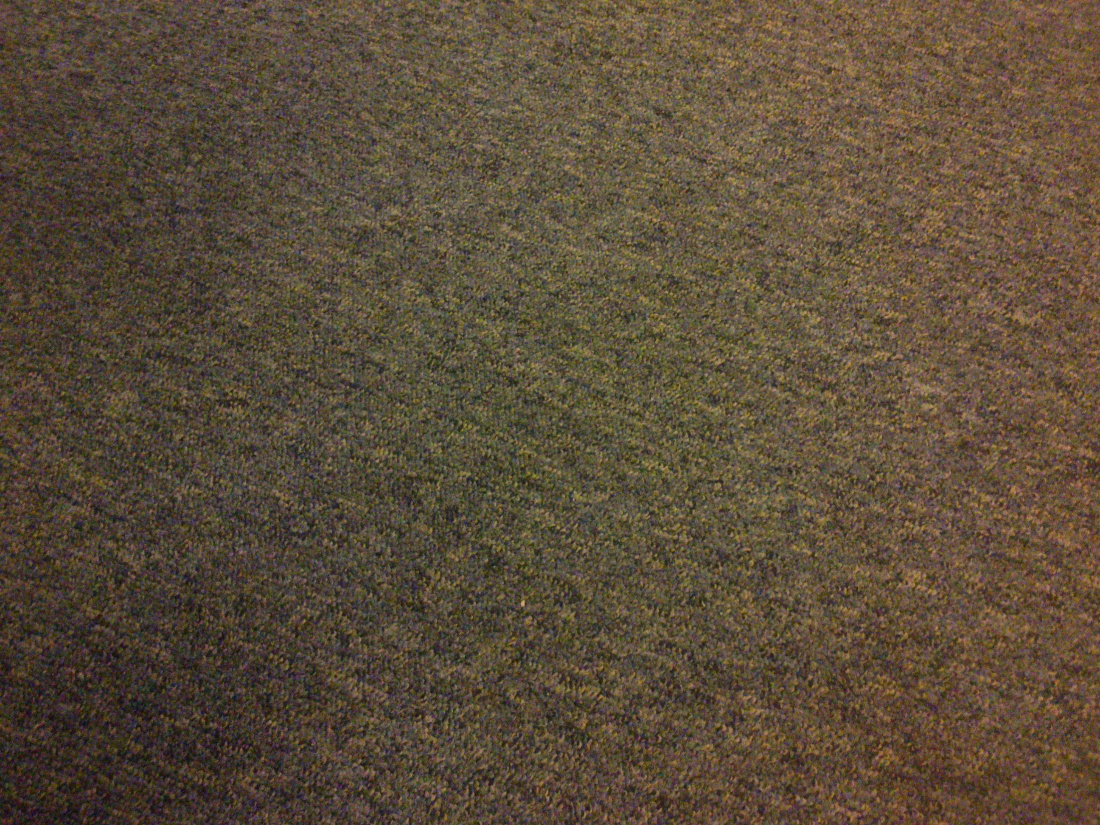
\includegraphics[width=4.5cm]{img/bad_input2}
\caption{The right image of the input image.} \label{x2}
\end{subfigure}
\begin{subfigure}[b]{0.45\textwidth}
\centering
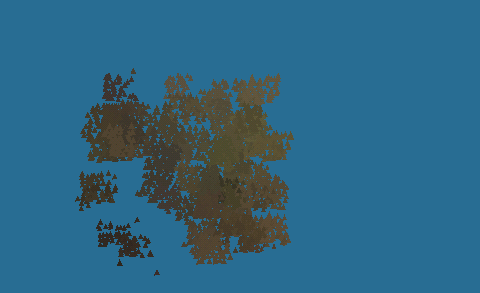
\includegraphics[width=5.0cm]{img/bad_result.png}
\caption{The result of the pair of images.} \label{x3}
\end{subfigure}
\caption[]{An example of a pair of images resulting in a non-realistic model.} 
\label{fig:bad_example}
\end{figure}
Furthermore, when testing our application we have experimented with some parameters, as illustrated by Figure \ref{fig:matching_comparison}, which demonstrates how the number of mismatches depends on the size of the rectangular box utilized in the second SURF matching described in section \ref{sec:matching}.
\begin{figure}[H]
\centerline{
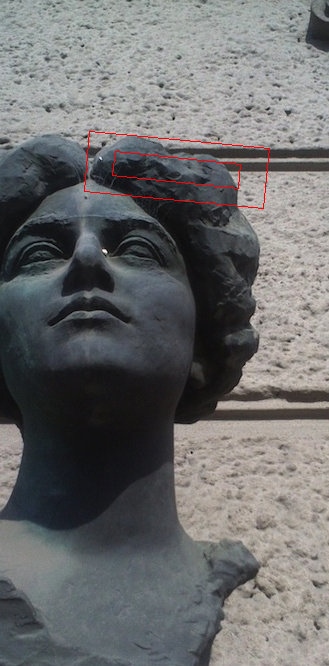
\includegraphics[width=3.42cm]{img/rectangle_w_02_h_035_croped.png}
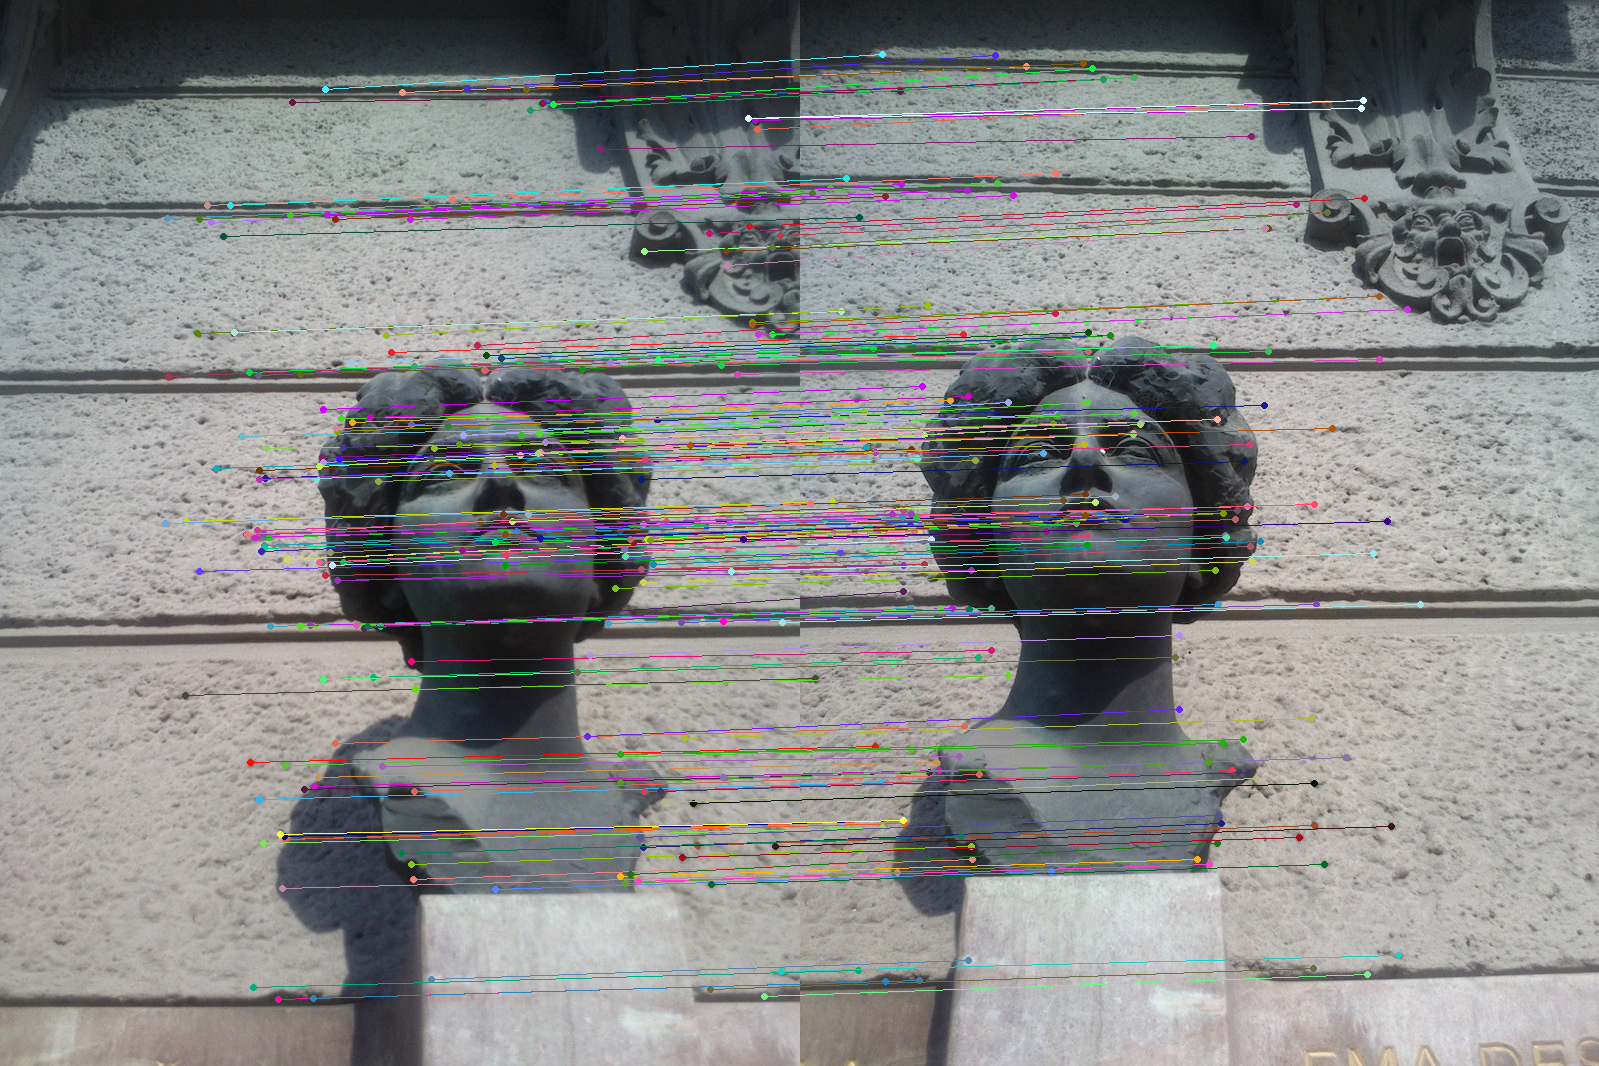
\includegraphics[width=10.4cm]{img/matching_w_02_h_035.png}}
\centerline{
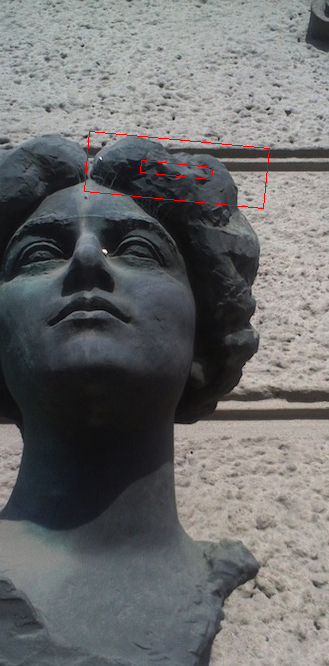
\includegraphics[width=3.42cm]{img/rectangle_w_01__h_02_croped.png}
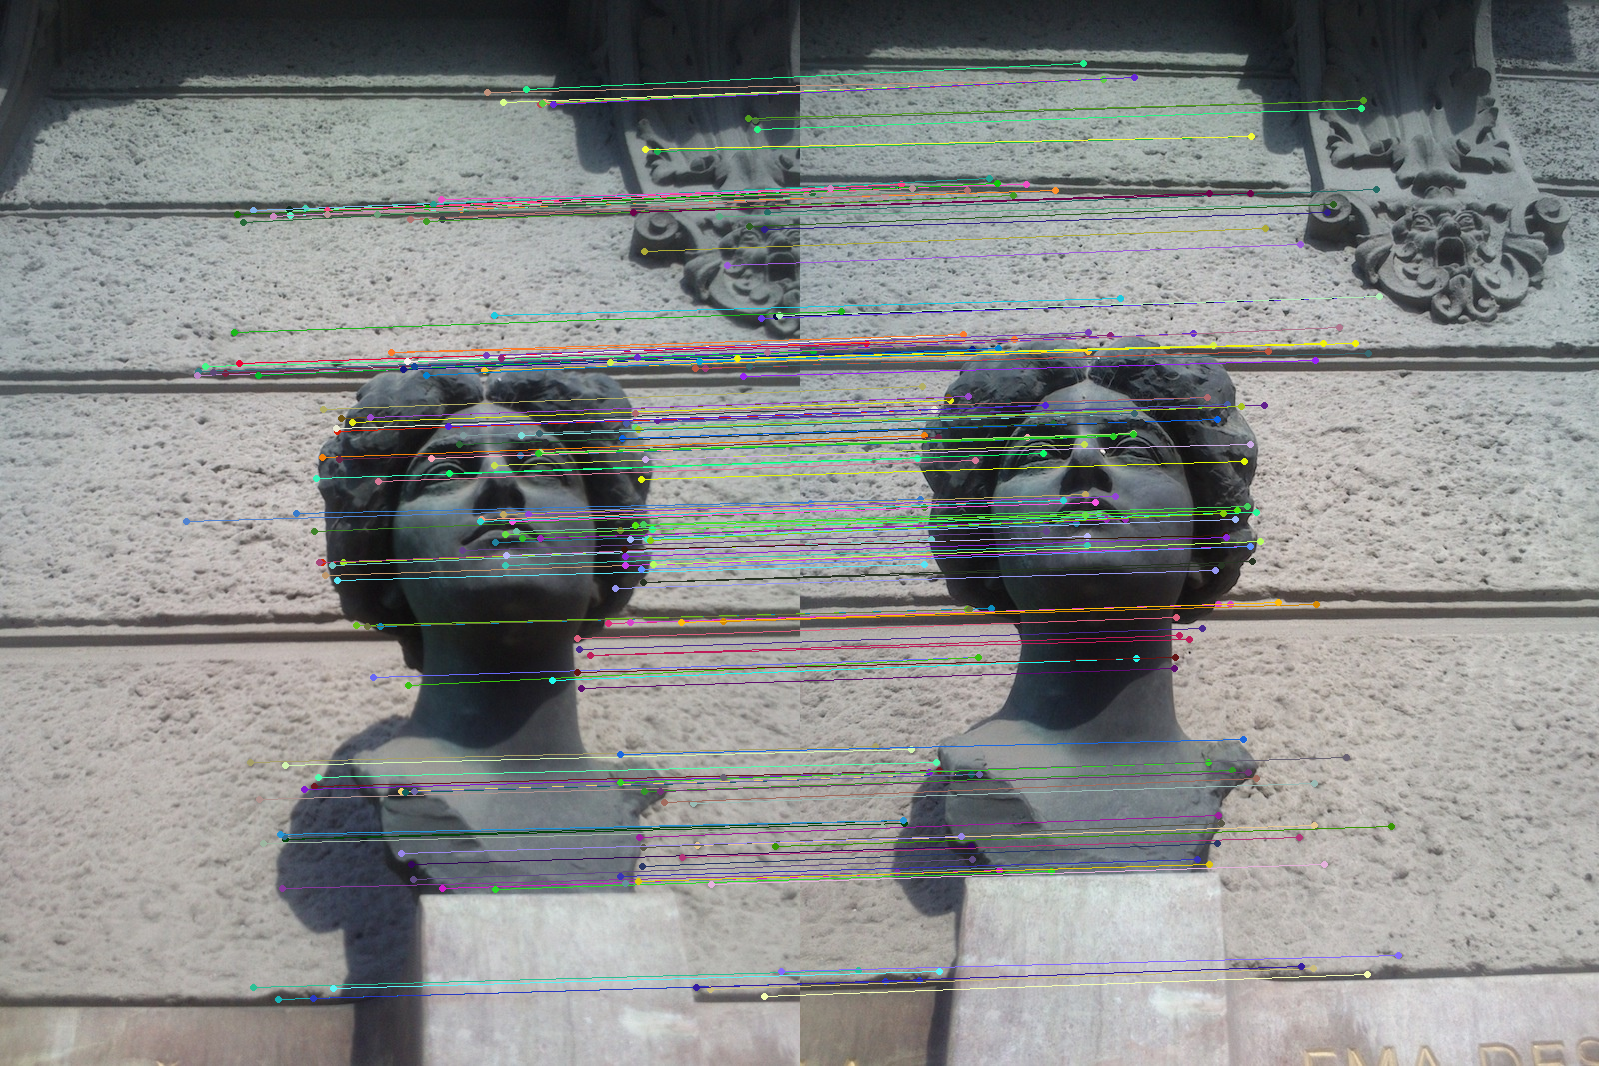
\includegraphics[width=10.4cm]{img/matching_w_01_h_02.png}}
\caption{A comparison of the result of matching with different sizes of the oriented rectangles. 
At the top left, there is a sample of the oriented rectangle where the width of inner rectangle is 20\% and height is 35\% of the size of the large one. 
Next to them are the corresponding results of SURF matching where for each feature in the first image, we estimate the rectangles and apply the inner one as described in Section \ref{sec:matching}.
We can see that in the bottom case there are fewer mismatches than in the top one.}
\label{fig:matching_comparison}
\end{figure}


